\documentclass[journal=jpcl,manuscript=letter,layout=traditional]{achemso}
\usepackage{amsmath,xcolor,graphicx,colortbl}
\usepackage{amssymb,soul,color}

\author{George Volonakis}\altaffiliation{These authors contributed equally to this work}
\affiliation[Department of Materials, University of Oxford]{Department of Materials, University of
Oxford, Parks Road OX1 3PH, Oxford, UK}

\author{Marina R. Filip} \altaffiliation{These authors contributed equally to this work}
\affiliation[Department of Materials, University of Oxford]{Department of Materials, University of
Oxford, Parks Road OX1 3PH, Oxford, UK}

\author{Amir Abbas Haghighirad}\affiliation[Department of Physics, University of Oxford]{Department of Physics,
University of Oxford, Clarendon Laboratory, Parks Road, Oxford OX1 3PU, UK}

\author{Nobuya Sakai}\affiliation[Department of Physics, University of Oxford]{Department of Physics,
University of Oxford, Clarendon Laboratory, Parks Road, Oxford OX1 3PU, UK}

\author{Bernard Wenger}\affiliation[Department of Physics, University of Oxford]{Department of Physics,
University of Oxford, Clarendon Laboratory, Parks Road, Oxford OX1 3PU, UK}

\author{Henry J. Snaith}\affiliation[Department of Physics, University of Oxford]{Department of Physics,
University of Oxford, Clarendon Laboratory, Parks Road, Oxford OX1 3PU, UK}
\email{feliciano.giustino@materials.ox.ac.uk}\phone{(+44) 1865 612790 }

\author{Feliciano Giustino} \affiliation[Department of Materials, University of Oxford]{Department of
Materials, University of Oxford, Parks Road OX1 3PH, Oxford, UK}
\email{henry.snaith@physics.ox.ac.uk}\phone{(+44) 01865 272380 }



\title{Lead-Free Halide Double Perovskites via Heterovalent Substitution of Noble Metals}


\begin{document}
\newpage

\begin{abstract}

Lead-based halide perovskites are emerging as the most promising class of materials for next generation
optoelectronics. However, despite the enormous success of lead-halide perovskite solar
cells, the issues of stability and toxicity are yet to be resolved. Here
we report on the computational design and the experimental synthesis of a new family of Pb-free
inorganic halide double-perovskites based on bismuth or antimony and noble metals. Using
first-principles calculations we show that this hitherto unknown family of perovskites
exhibits very promising optoelectronic properties, such as tunable band gaps in the visible range and
low carrier effective masses. Furthermore, we successfully synthesize the
double perovskite Cs$_2$BiAgCl$_6$, perform structural refinement using
single-crystal X-ray diffraction, and characterize its optical properties via optical absorption
and photoluminescence measurements. This new perovskite belongs to the $Fm\bar{3}m$ space group,
and consists of BiCl$_6$ and AgCl$_6$ octahedra alternating in a rock-salt face-centered cubic structure.
From UV-Vis and PL measurements we obtain an indirect gap of 2.2~eV.\\

\end{abstract}


\newpage


Perovskites are among the most fascinating crystals, and play important
roles in a variety of applications, including ferroelectricity, piezoelectricity, high-T$_{\rm c}$
superconductivity, ferromagnetism, giant magnetoresistance, photocatalysis and photovoltaics~\cite{Suntivich2011,
Stranks2015, Gratzel2014, Vasala2015,
Grinberg2013, Ramesh2007, Rinjders2005, Ahn2004}. The majority of perovskites are oxides
and are very stable under ambient temperature and pressure conditions~\cite{Vasala2015, Fan2015}.
However, this stability is usually accompanied by very large band gaps, therefore most oxide perovskites
are not suitable candidates for optoelectronic
applications. The most noteworthy exceptions are the ferroelectric perovskite oxides related to LiNbO$_3$,
BaTiO$_3$, Pb(Zr, Ti)O$_3$ and BiFeO$_3$, which are being actively investigated for photovoltaic applications, reaching
power conversion efficiencies of up to 8\%\cite{Fan2015}.
The past five years witnessed a revolution in optoelectronic research with the discovery of the organic-inorganic
lead-halide perovskite family. These solution-processable perovskites are fast becoming the most promising materials
for the next generation of solar cells, achieving efficiencies above 20\%~\cite{Green2014, Lee2012,
Kim2012, NREL}. Despite this breakthrough, hybrid lead-halide perovskites are known to degrade due to moisture and
heat~\cite{Manser2016}, upon prolonged exposure to light,~\cite{Hoke2015} and are prone to ion or halide vacancy migration,
leading to unstable operation of photovoltaic devices~\cite{Eames2015, Meloni2016}. At the same time the presence of lead
raises concerns about the potential environmental impact of these materials~\cite{Espinosa2015, Babagayigit2016}. Given
these limitations, identifying a stable, non-toxic halide perovskite optoelectronic material is one of the key  challenges
to be addressed in the area of perovskite optoelectronics.

The starting point of our search for a lead-free halide-perovskite is the prototypical inorganic compound CsPbI$_3$. CsPbI$_3$
is an ABX$_3$ perovskite where the heavy metal cations Pb$^{2+}$ and the halide anions I$^-$ occupy the B and X sites,
respectively, while Cs$^+$ occupies the A site. The most obvious route to replacing Pb in this compound is via substitution
of other group-14 elements such as Sn and Ge. However both elements tend to undergo oxidation, for example from Sn$^{2+}$
to Sn$^{4+}$, leading to a rapid degradation of the corresponding halide perovskites~\cite{Stoumpos2013, Baikie2013,
Hao2014, Noel2014}. More generally, it should also be possible to substitute lead by other divalent cations outside of
group-14 elements. However, our previous high-throughput computational screening  of potential candidates showed that the
homovalent substitution of lead in halide perovskites impacts negatively the optoelectronic properties by increasing band
gaps and effective masses~\cite{Filip2016}.

Another possible avenue is to consider heterovalent substitution, that is the formation of a double perovskite structure with
a basic formula unit A$_2$B$^\prime$B$^{\prime\prime}$X$_6$~\cite{Vasala2015}. This type of compounds are abundant in the case of oxides
and are well known for their ferroelectric, ferromagnetic and multiferroic properties~\cite{Vasala2015}.
Additionally, double perovskites have been explored in order to tune the band gap of oxide perovskites~\cite{Nechache2015, Berger2012}.
On the other hand,  halide double perovskites remain a much less explored class of materials. To date, the best
known halide double perovskites are based on alkali and rare-earth metals, and are investigated for applications as
scintillators in radiation detectors~\cite{Loef2002}.

In order to replace the divalent Pb cations and maintain the total charge neutrality, the B$^\prime$ and B$^{\prime\prime}$ sites
have to be occupied by one monovalent and one trivalent cation. We search for our B$^{\prime3+}$ metallic cations among the pnictogens,
and consider Bi and Sb as the most suitable choices. Arsenic is less desirable owing to its toxicity. For the monovalent cations
we choose the noble metals Cu, Ag and Au. From elementary considerations Cu, Ag, and Au appear very promising for optoelectronic
applications. In fact, in their metallic form, the noble metals are the best known electrical conductors, owing to their filled
$d^{10}$ shell and the free-electron-like behaviour of the $s^1$ shell. In addition, in an octahedral environment, the ionic radii
of Cu$^+$ (0.91~\AA), Ag$^+$ (1.29~\AA) and Au$^+$ (1.51~\AA) are similar to those of Pb$^{2+}$ (1.19~\AA), Sb$^{3+}$ (0.76~\AA)
and Bi$^{3+}$ (1.03~\AA)~\cite{Shannon}. We note that the cost of the precursors for the proposed Pb-alternatives (AgCl and CuCl) are similar to the case of lead, except for the case of gold (AuCl) which is considerably more expensive. Following this simple
reasoning we investigate hypothetical halide double perovskites with the pairs B$^\prime$/B$^{\prime\prime}$ where B$^\prime$ =
Sb, Bi, and B$^{\prime\prime}$ = Cu, Ag, Au.

We investigate the electronic properties of these hypothetical compounds from first principles using density functional theory (DFT) in the local density approximation (LDA).
We construct `rock-salt' double perovskites, whereby B$^\prime$ and B$^{\prime\prime}$ alternate in every direction (shown
in Figure~\ref{fig:1}a). The rock-salt ordering is known to be the ground state for most oxide double perovskites~\cite{Vasala2015},
therefore it can be expected to hold also in the present case. For each model structure we perform full structural optimization
using DFT-LDA and calculate the electronic band gaps using the hybrid PBE0 functional as described in the Supporting Information.

\begin{figure}[t!]
\begin{center}
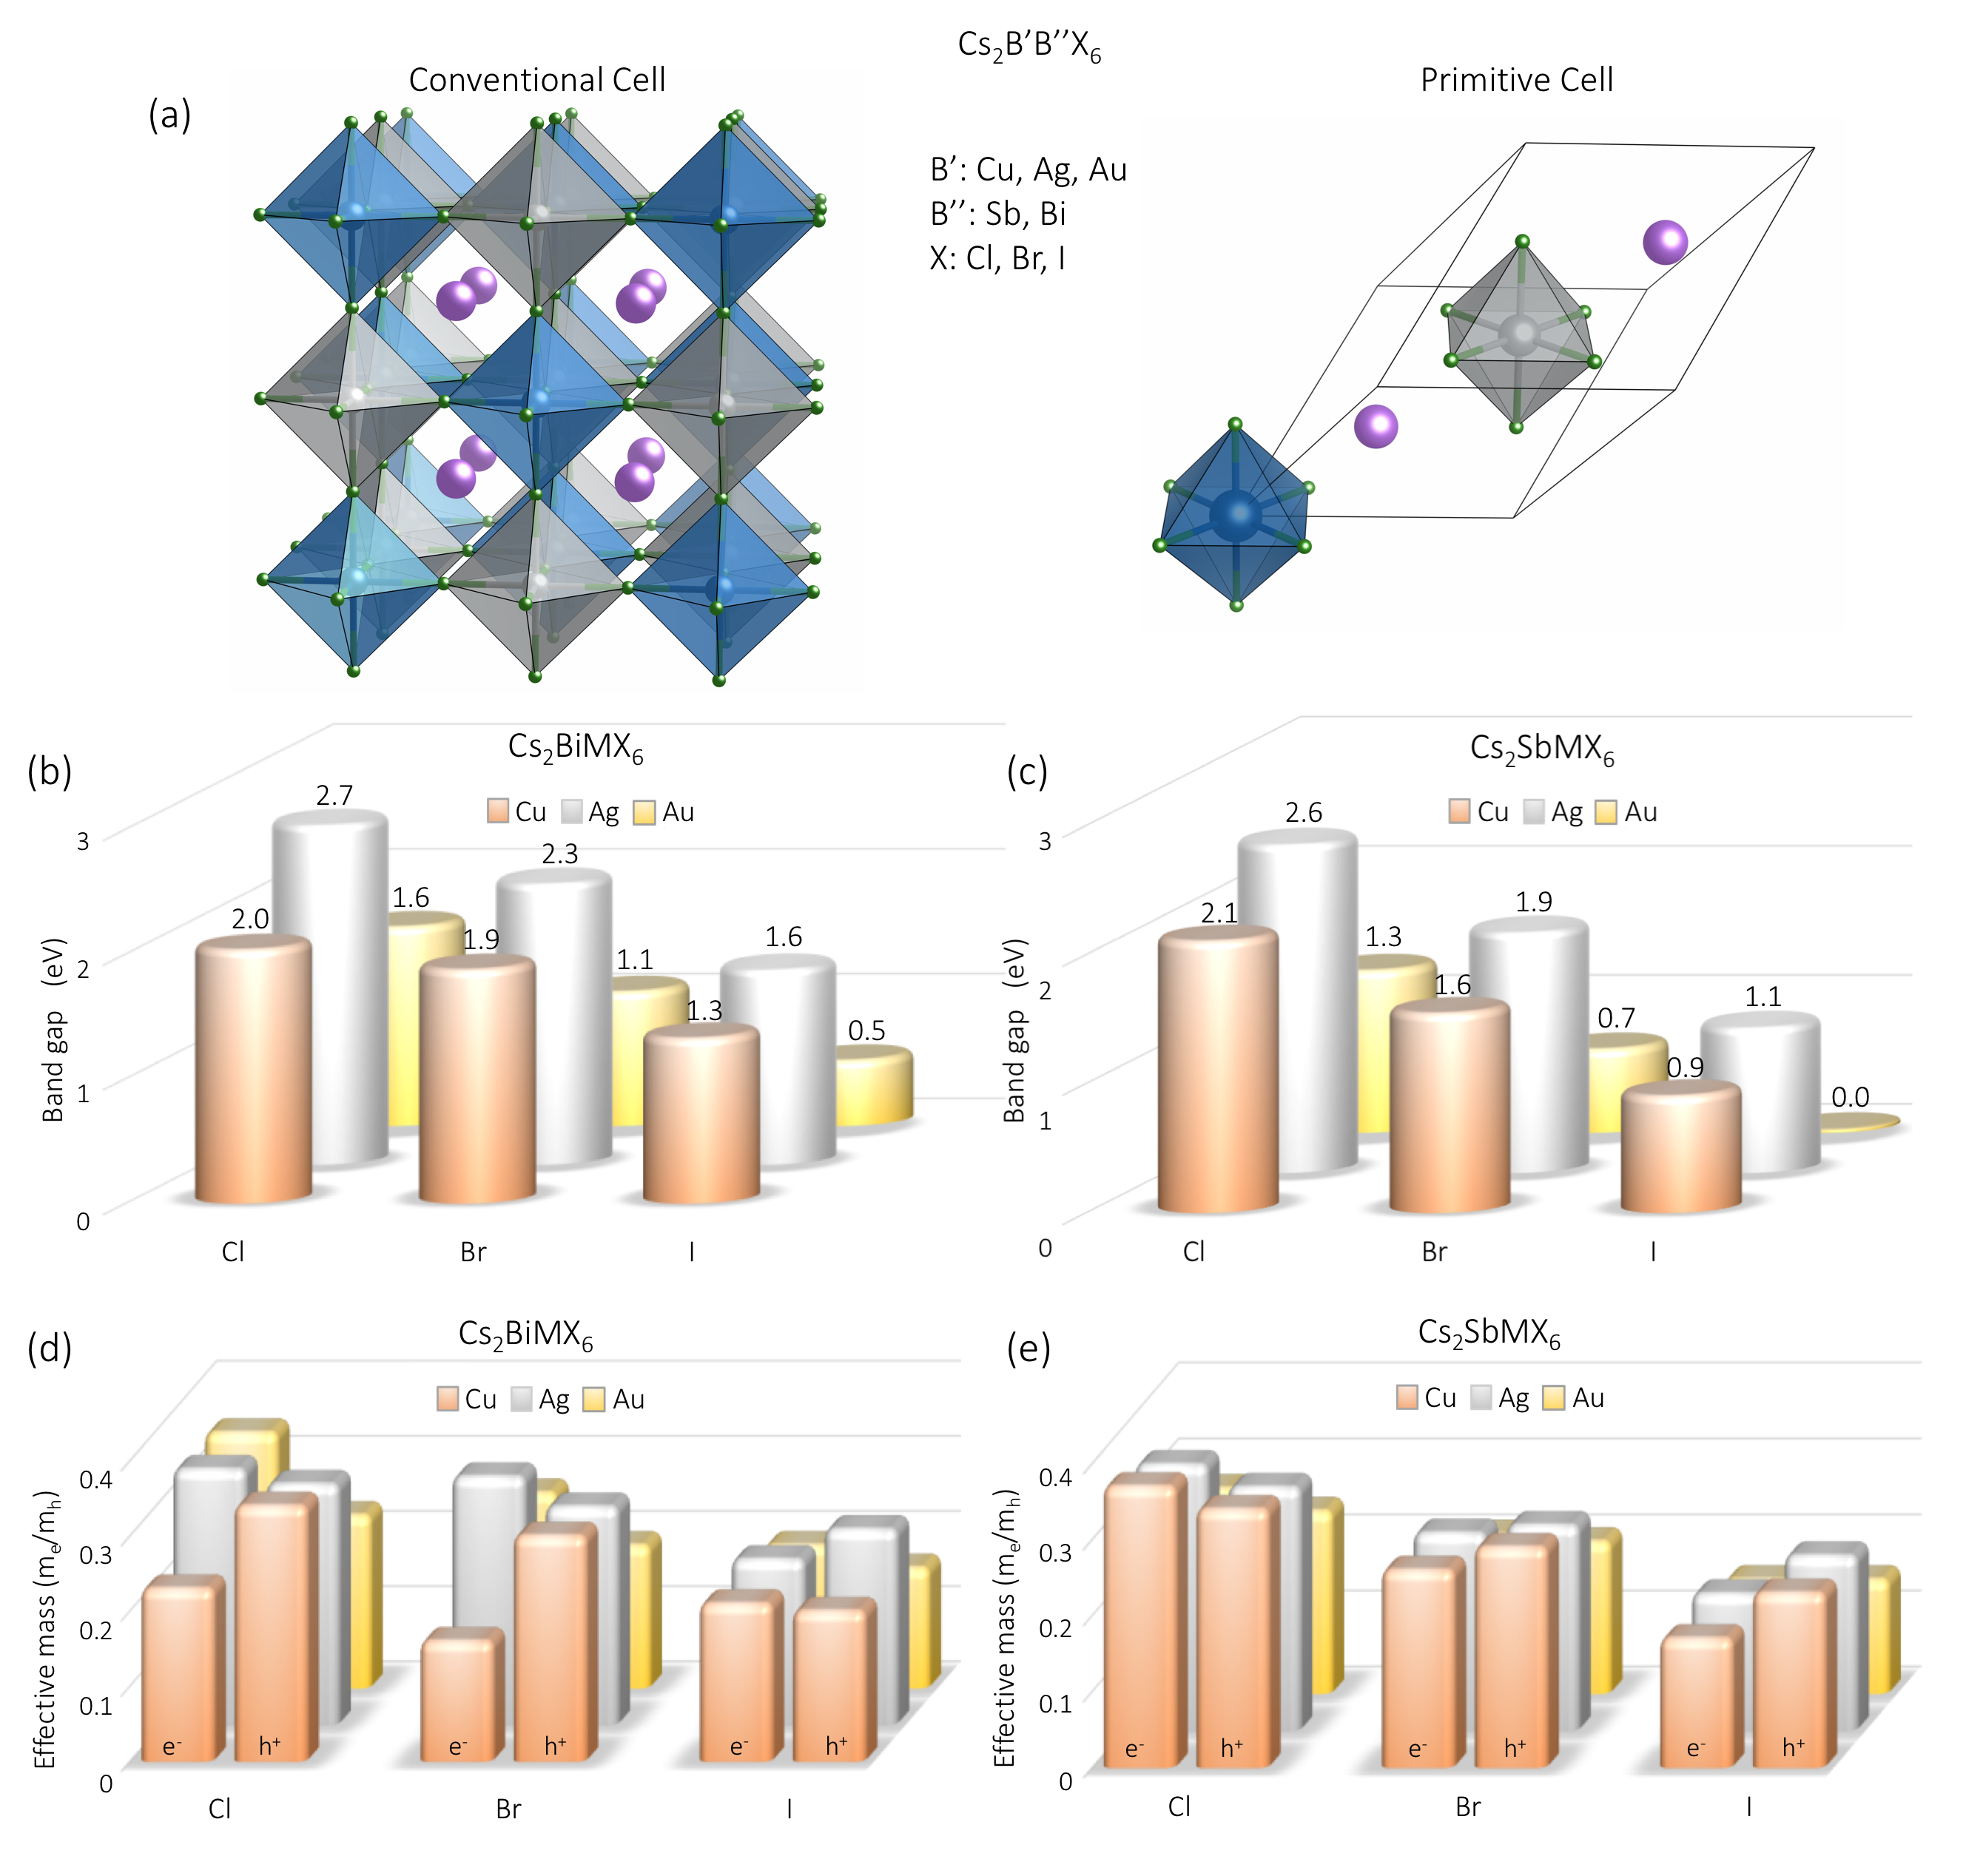
\includegraphics[width=0.94\textwidth]{fig1.png}
\end{center}
\caption{\label{fig:1}
  \textbf{Computational screening of the electronic properties of the pnictogen-noble metal halide double perovskites\hspace{0.2cm}}\\
  \textbf{a}~Polyhedral model of the conventional (left) and reduced (right) unit cell of the hypothetical halide double perovskites.
  The pnictogen (B$^\prime$) and noble metal (B$^{\prime\prime}$) cations alternate along the three crystallographic axes, forming
  the rock-salt ordering.
  \textbf{b}~Electronic  band gaps calculated for all compounds in the halide double perovskite family using the PBE0 hybrid functionals.
  All calculated band gaps are indirect with the top of the valence band at the X point (0,0,$2\pi/a$) of the Brillouin zone, where $a$ is
  the lattice parameter of the FCC unit cell. The bottom of the conduction band is at the L point ($\pi/a$, $\pi/a$, $\pi/a$) of the
  Brillouin zone in all cases, except Cs$_2$BiAgCl$_6$, Cs$_2$BiCuCl$_6$ and Cs$_2$BiCuBr$_6$ where the bottom of the conduction band
  is found at the $\Gamma$ (0,0,0) point.
  \textbf{c}~Conductivity effective masses calculated from DFT/LDA for each compound (see Supporting Information). The effective masses
  are calculated at the VBM (holes) and CBM (electrons)  in each case.
}
\end{figure}


In Figure~\ref{fig:1}b-c we show a comparative view of the band gaps calculated for the entire Cs$_2$B$^\prime$B$^{\prime\prime}$X$_6$ family.
We find that all band gaps are below 2.7~eV, spanning the visible and near infrared optical spectrum. The band gaps are
indirect and increase as we move up the halogen or the pnictogen column in the periodic table, but do not follow a monotonic
trend with respect to the size of the noble metal cation. This behaviour can be explained by the character of the electronic
states at the band edges. Indeed, a shown in Figure~S1 of the Supporting Information, the conduction band bottom and
valence band top in each case are predominantly of pnictogen-$p$ and halogen-$p$ character, respectively. As we move up in
the periodic table the energy of the halogen-$p$ states decreases, thus lowering the energy of the valence band top. Similarly,
the energy of the pnictogen-$p$ states decreases when moving up in the periodic table, thus lowering
the energy of the conduction band bottom. The electron and hole effective masses calculated at the band edges exhibit an
anisotropic behaviour in most cases (see Table~S1). Throughout the entire family of compounds the electron masses are more isotropic than the hole masses. For clarity, in
Figure~\ref{fig:1} we report the conductivity effective masses~\cite{Galli2014}, as defined in the Supporting Information.
We note that all compounds exhibit small carrier effective masses between 0.1 and 0.4~$m_e$, very close to those calculated
for CH$_3$NH$_3$PbI$_3$ within the same level of theory~\cite{Filip2015-2}.


The electronic band structures of these  halide double perovskites (shown in Figure S2 and S3) exhibit
several features of particular interest. In all cases, the valence band maximum (VBM) is at the $X$ (0,0,$2\pi/a$) point in the Brillouin
zone. The conduction band minimum (CBM) is at  $\Gamma$ (0,0,0) for Cs$_2$BiAgCl$_6$, Cs$_2$BiCuCl$_6$ and Cs$_2$BiCuBr$_6$, while
for the other compounds the CBM is at the $L$ ($\pi/a$, $\pi/a$, $\pi/a$) point.
In Figure~S4, we show the band structure of Cs$_2$BiAgCl$_6$  calculated in the conventional unit cell (which corresponds to four primitive cells and contains 8 octahedra in a cubic lattice). Here, as a result of Brillouin zone folding, the band gap of Cs$_2$BiAgCl$_6$  becomes direct at the $\Gamma$-point, although the direct transition is still forbidden by symmetry. This suggests an avenue for engineering a direct band gap in these compounds. In fact symmetry can be broken by inducing octahedral tilts, and this could be achieved by varying the steric size of the A-site cation (Cs)~\cite{Filip2014-1}. For example, this effect could be realized by incorporating an organic cation, like methylammonium or formamidinium into the cuboctahedral cavity. In order to demonstrate this point, we report in Figure S5 the calculated band structure of the hypothetical orthorhombic compound MA$_2$BiAgCl$_6$ (MA = CH$_3$NH$_3$, methylammonium; the structure is constructed as described in the Supporting Information). Explicit calculations of the optical matrix elements indicate that the direct optical transition in the methylammonium-based compound is  allowed, as expected.


\begin{figure}[t!]
\begin{center}
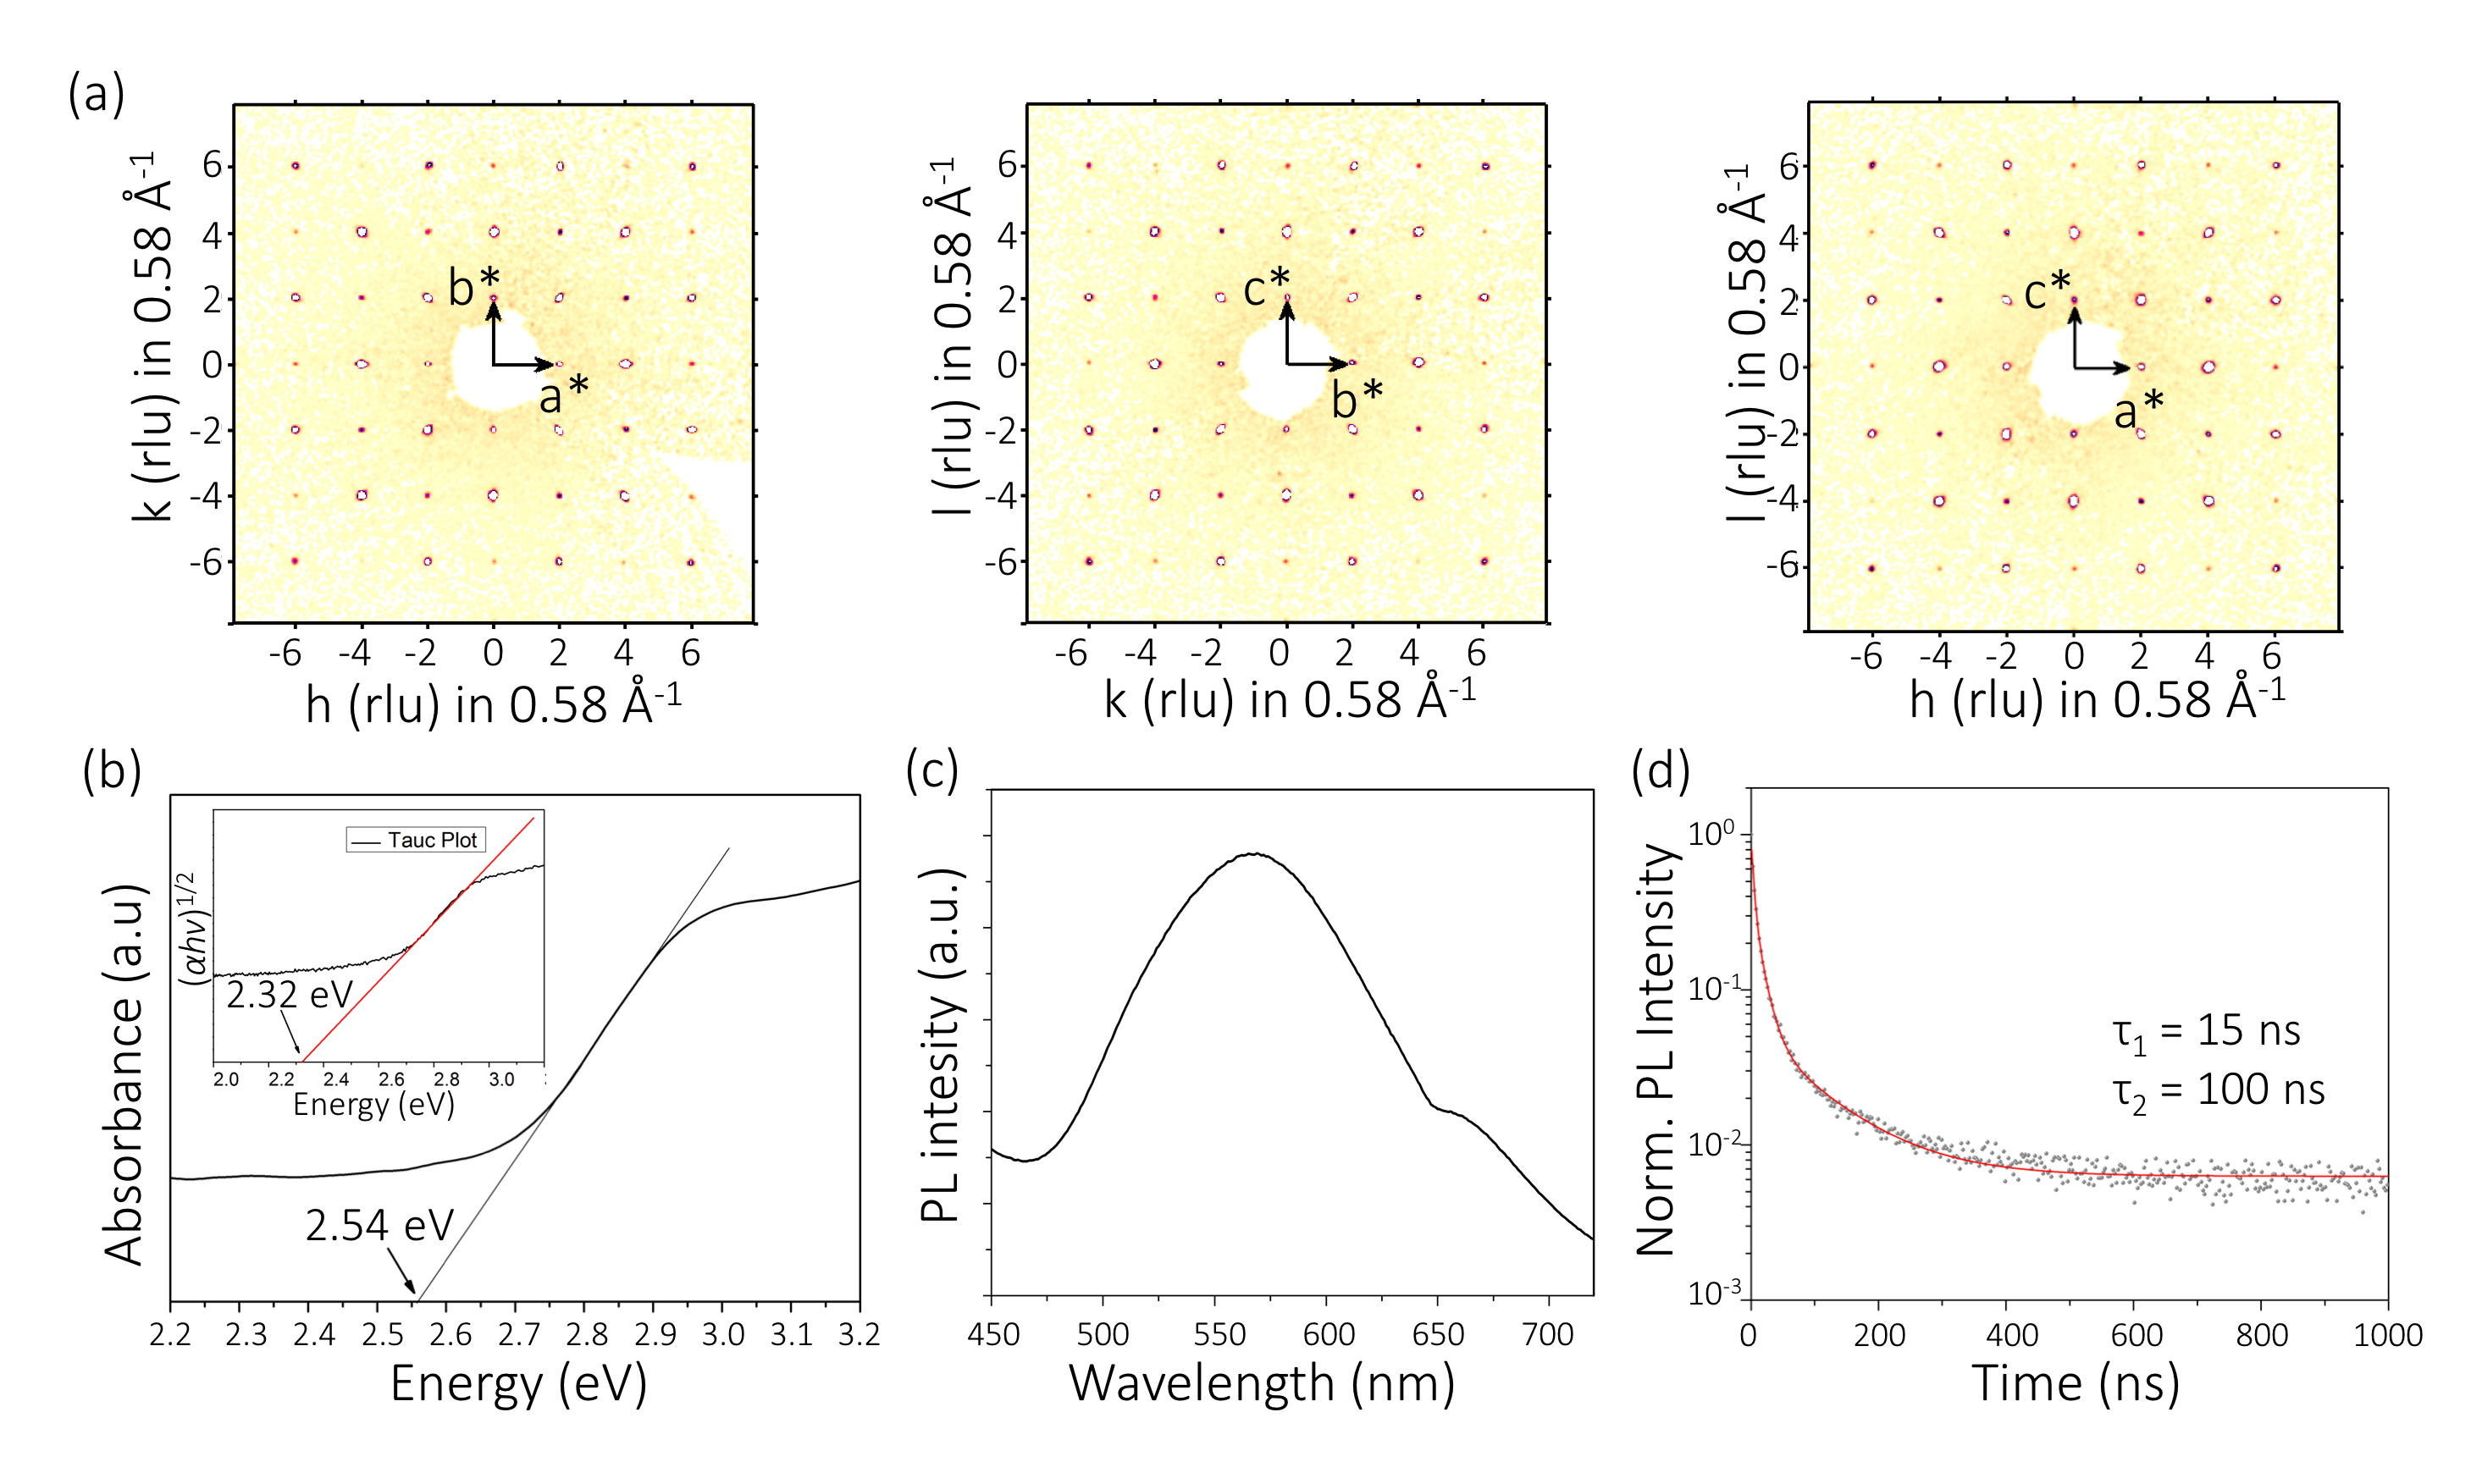
\includegraphics[width=1.0\textwidth]{fig2.png}
\end{center}
\caption{\label{fig:2}
 \textbf{Experimental synthesis and characterization of Cs$_2$BiAgCl$_6$.}\\
 \textbf{a} X-ray diffraction pattern for a Cs$_2$BiAgCl$_6$ single crystal at 293 K. $hkl$ shown for three different planes,
 i.e.  $0kl$, $h0l$ and $hk0$. All wave vectors are labeled in reciprocal lattice units (rlu) and  a$^\mathrm{*}$, b$^\mathrm{*}$
 and c$^\mathrm{*}$ denote reciprocal lattice vectors of the cubic cell of the $Fm\bar{3}m$ structure.
 \textbf{b} UV-Vis optical absorption spectrum of Cs$_2$BiAgCl$_6$. The inset shows the Tauc plot, corresponding to an indirect
 allowed transition [assuming the expression: $(\alpha h\nu)^{1/2} = C(h\nu - E_g)$, where $\alpha$ is the absorption coefficient,
 $h\nu$ is the energy of the incoming photon $E_g$ is the optical band gap and $C$ is a constant]. The straight lines are fitted to the
 linear regions of the absorption spectrum and Tauc plot, and the intercepts at 2.32~eV and 2.54~eV marked on the plot are calculated from the fit.
 \textbf{c} Steady-state photoluminescence (PL) spectrum of Cs$_2$BiAgCl$_6$, deposited on glass.
 \textbf{d} Time resolved photoluminescence decay of Cs$_2$BiAgCl$_6$, deposited on glass. The data is fitted using a biexponential decay
 function. The decay lifetimes of 15~ns (fast) and 100~ns (slow) is estimated from the fit.
}
\end{figure}


Having established that the family of  A$_2$B$^\prime$B$^{\prime\prime}$X$_3$  halide double perovskites, based on B$^\prime$ = Sb, Bi and B$^{\prime\prime}$ = Cu,
Ag, Au exhibits promising optoelectronic properties, we move to the synthesis and optical characterization of a representative member of
this group of compounds. We adapt the synthesis process of Cs$_2$BiNaCl$_6$, reported in Ref.~\cite{Morss1972},
to allow for the incorporation of a noble metal. Of the three noble metals under consideration, Ag has an ionic radius
which is closest to that of Na (1.02~\AA\ vs 1.15~\AA). For this reason we proceed to synthesize Cs$_2$BiAgCl$_6$ by conventional solid-state
reaction as described in detail in the Supporting Information. In Figure~\ref{fig:2}a we show the X-ray Diffraction Pattern for
a single crystal ($\sim$30$\mu$m  diameter). We observe sharp reflections for the crystallographic $0kl$, $h0l$ and $hk0$ planes. These reflections show
characteristics of $m$$\bar{3}$$m$ symmetry that reveal systematic absences for ($hkl$; $h+k$, $k+l$, $h+l = 2n$) corresponding to the face-centered space groups $F432$,
$F\bar{4}3m$ and $Fm\bar{3}m$. The latter was selected for structure refinement after confirmation that Cs$_2$BiAgCl$_6$ crystallizes in an FCC
lattice. We find that there is no significant distortion of octahedral symmetry about the Bi$^{3+}$. The atomic
positions from the structural refinement are listed in Table~S2 of the Supplementary Information. The X-ray diffraction patterns uniquely
identify the $Fm\bar{3}m$ (no. 225) space group at room temperature, and the quantitative structural analysis gives a very good description of the data. In addition, our crystal structure refinement is  consistent with the rock-salt configuration
assumed by our atomistic model. The experimental and computationally predicted conventional lattice parameters are in very good agreement, 10.78~\AA\
and 10.50~\AA, respectively.
From the optical absorption spectrum and Tauc plot (see Figure~\ref{fig:2}b) we can estimate an indirect optical band gap in the range
of 2.3-2.5~eV. The indirect character of the band gap is consistent with the broad photoluminescence peak observed between 480 and 650 nm (1.9-2.6~eV)
with the maximum at $\sim$575~nm (2.2~eV), red-shifted with respect to the optical absorption onset. In addition, the  time-resolved
photoluminescence decay shown in Figure~\ref{fig:2}c was fitted with a double exponential giving a fast component
lifetime of 15~ns and a slow component lifetime of 100~ns.The as-made compound appears to be stable under ambient conditions for weeks after synthesis, with the bright yellow color persisting and no visible changes appearing in the powder X-ray diffraction patterns (see Figures~S6 and S7).




\begin{figure}[t!]
\begin{center}
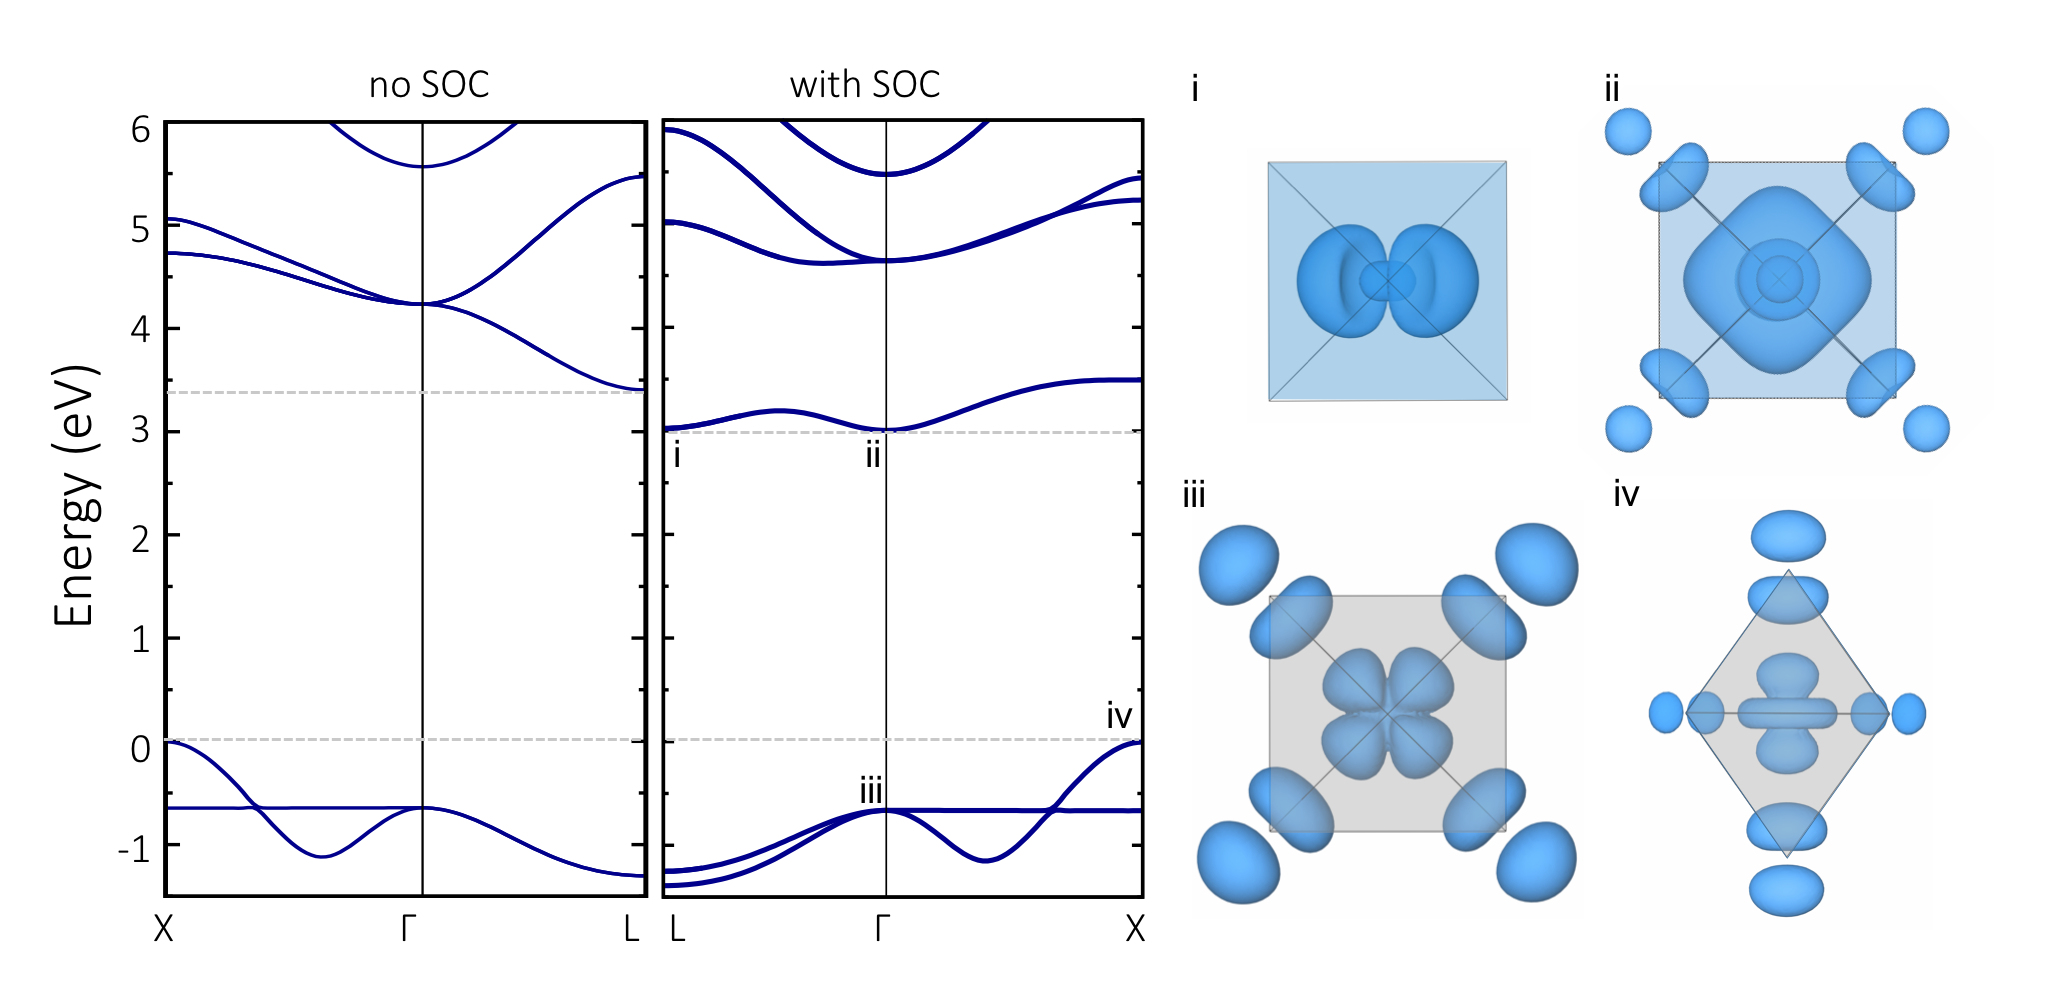
\includegraphics[width=1.0\textwidth]{fig3.png}
\end{center}
\caption{\label{fig:3}
  \textbf{Electronic structure properties calculated for the experimental crystal structure of Cs$_2$BiAgCl$_6$.}\\
  The Band structure of Cs$_2$BiAgCl$_6$ calculated along the high symmetry path L($\pi/a, \pi/a, \pi/a$) - $\Gamma$ (0,0,0)
  - X (0,0,2$\pi$/a) without (left) and with (right) spin-orbit coupling.
  The black points on the fully relativistic band structure marked `i-iv' mark the conduction band bottom at L
  and $\Gamma$ and the valence band top at $\Gamma$ and X, respectively. For each of the states we show the electronic wavefunctions. The   conduction band bottom is primarily of
  Bi-$p$ and Cl-$p$ character, while the valence band top consists of Ag-$d$ and Cl-$p$ character. The shape of all
  four wavefunctions is consistent with metal-halide $\sigma$-bonds.
}
\end{figure}

In Figure~\ref{fig:3} we show the electronic band structure of Cs$_2$BiAgCl$_6$ calculated for the as determined experimental crystal structure,
with and without relativistic spin-orbit coupling effects. The features of the valence band edge are almost unchanged
when the relativistic effects are included. This is consistent with the predominant Cl-$p$ and Ag-$d$ character of this band.
By contrast, due to the large spin-orbit coupling, the conduction band edge splits in two bands, separated by more than 1.5~eV at the $\Gamma$ point.
This effect is not surprising, given that the character of the conduction band bottom is
of primarily Bi-$p$ character. For comparison, in the case of Cs$_2$SbAgCl$_6$ (see Figure~S8) the
spin-orbit splitting of the conduction band at the $\Gamma$ point is of only 0.5~eV. The fundamental band gap is reduced by 0.4~eV
upon inclusion of relativistic effects, and the shape of the conduction band is drastically different. Therefore, the inclusion
of spin-orbit coupling is crucial for the correct description of the conduction band edge, bearing resemblance to the
case of CH$_3$NH$_3$PbI$_3$~\cite{Even2013,  Filip2014-2}. In the fully relativistic case we calculated an indirect band gap of
3.0~eV and lowest direct transition of 3.5~eV, in very close agreement  with the results obtained for the model Cs$_2$BiAgCl$_6$ structure,
discussed in Figure~\ref{fig:1} [2.7~eV (indirect) and 3.3~eV (direct)]. The small difference in band gap of 0.2-0.3~eV is due to the
small difference in volume between the experimental and predicted crystal structure. The calculated electronic
band gaps are overestimated with respect to the measured optical band gap by approximately 0.5~eV. This quantitative discrepancy does not
affect the qualitative physical trends of the band gaps discussed throughout this work, and can be associated to the approximations
employed in our PBE0 calculations. A better agreement with experiment can be reached by fine-tuning the fraction of exact
exchange, or by performing $GW$ calculations~\cite{Hedin, Hybertsen}. The latter will be reported in a future work.


In summary, through a combined theoretical and experimental study, we have designed a new family of halide double-perovskite semiconductors based on pnictogens and noble metals. We used state-of-the-art first-principles calculations in order to explore trends in the electronic and optical properties in the entire family of double perovskites A$_2$B$^\prime$B$^{\prime\prime}$X$_6$ with A = Cs, B$^\prime$ = Bi, Sb, B$^{\prime\prime}$ = Cu, Ag, Au, and X = Cl, Br, I. Our calculations revealed highly tunable carrier effective masses, and optical gaps across the visible range of the electromagnetic spectrum. We predicted all compounds to be indirect gap semiconductors, and proposed a simple strategy for turning them into direct-gap materials. We successfully synthesized Cs$_2$BiAgCl$_6$, and obtained a face-centered cubic double perovskite. Optical characterization confirmed our theoretical predictions, indicating an indirect gap semiconductor. Overall, the present work is the first detailed description of the structure and optoelectronic properties of the pnictogen-noble metal halide double perovskite family, and calls for many future experimental and theoretical studies in order to assess the full potential of these new materials. We expect that a complete mapping of the genome of halide double perovskites based on pnictogens and noble metals may unlock a world of new functional materials for photovoltaics, photocatalysis, photodetectors, light-emitting devices, piezoelectrics, and magnetoelectrics.

\vspace{0.6cm}

\noindent {\bf Supporting Information Available:} Description of the computational setup, details on the materials synthesis and characterization and crystallographic data. All the electronic band structures for the pnictogen-noble metal double halide perovskites. Additional figures relevant to the discussions in this article. This material is available free of charge via the Internet http://pubs.acs.org.

\begin{acknowledgement}
The research leading to these results has received funding from the the Graphene Flagship
(EU FP7 grant no. 604391), the Leverhulme Trust (Grant RL-2012-001), the UK Engineering and Physical
Sciences Research Council (Grant No. EP/J009857/1 and EP/M020517/1), and the European Union Seventh Framework
Programme (FP7/2007-2013) under grant agreements n$^\circ$239578 (ALIGN) and n$^\circ$604032 (MESO).
The authors acknowledge the use of the University of Oxford Advanced
Research Computing (ARC) facility (http://dx.doi.org/
10.5281/zenodo.22558) and the ARCHER UK National
Supercomputing Service under the `AMSEC' Leadership project. G.V., M.R.F. and F.G. would like to thank Marios
Zacharias for useful discussions. Figures involving atomic structures were rendered using VESTA \cite{VESTA}.
\end{acknowledgement}


\vspace{0.6cm}

\noindent
 {\large \bf Note added}

\noindent
During the preparation of this manuscript we became aware of the publication of two related papers: Ref.~\cite{Slavney2016} (published
February 7th, 2016) and Ref.~\cite{McClure2016} (published February 10th, 2016). The key difference between the present
work and that of Ref.~\cite{Slavney2016, McClure2016} is that we perform a computational screening of the entire family
of pnictogen-noble metal double halide perovskites and perform experiments that confirm our predictions.
\bibliography{bibliography}


\end{document}
